\documentclass{standalone}

\usepackage{tikz}
\usetikzlibrary{shapes.geometric}
\begin{document}
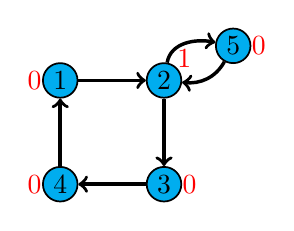
\begin{tikzpicture}
[every node/.style={inner sep=0pt}]
\node (1) [circle, minimum size=12.5pt, fill=cyan, line width=0.625pt, draw=black,label=left:$\color{red} 0$] at (25.0pt, -37.5pt) {\textcolor{black}{1}};
\node (2) [circle, minimum size=12.5pt, fill=cyan, line width=0.625pt, draw=black,label=above right:$\color{red} 1$] at (62.5pt, -37.5pt) {\textcolor{black}{2}};
\node (3) [circle, minimum size=12.5pt, fill=cyan, line width=0.625pt, draw=black,label=right:$\color{red} 0$] at (62.5pt, -75.0pt) {\textcolor{black}{3}};
\node (4) [circle, minimum size=12.5pt, fill=cyan, line width=0.625pt, draw=black,label=left:$\color{red} 0$] at (25.0pt, -75.0pt) {\textcolor{black}{4}};
\node (5) [circle, minimum size=12.5pt, fill=cyan, line width=0.625pt, draw=black,label=right:$\color{red} 0$] at (87.5pt, -25.0pt) {\textcolor{black}{5}};
\draw [line width=1.25, ->, color=black] (4) to  (1);
\draw [line width=1.25, ->, color=black] (1) to  (2);
\draw [line width=1.25, ->, color=black] (2) to  (3);
\draw [line width=1.25, ->, color=black] (3) to  (4);
\draw [line width=1.25, ->, color=black] (2) to  [in=169, out=80] (5);
\draw [line width=1.25, ->, color=black] (5) to  [in=354, out=241] (2);
\end{tikzpicture}
\end{document}
